\documentclass[11pt,letterpaper]{article}
\usepackage[lmargin=1in,rmargin=1in,tmargin=1in,bmargin=1in]{geometry}
\usepackage{../style/homework}
\usepackage{../style/commands}
\setbool{quotetype}{true} % True: Side; False: Under
\setbool{hideans}{false} % Student: True; Instructor: False

% -------------------
% Content
% -------------------
\begin{document}

\homework{13: Due 11/07}{Above all, don't fear difficult moments. The best comes from them.}{Rita Levi-Montalcini}

% Problem 1
\problem{10} Consider the linear function $f(x)= 7 - \frac{6}{7}\, x$.
	\begin{enumerate}[(a)]
	\item Find the rate of change of $f(x)$.
	\item Is $f(x)$ increasing or decreasing? Explain.
	\item Find the $y$-intercept of $f(x)$.
	\item Find $f(-3)$.
	\end{enumerate} \pspace

\sol 
\begin{enumerate}[(a)]
\item The rate of chance of a linear function is its slope. Because $f(x)= 7 - \frac{6}{7}\,x$ has the form $y= mx + b$ with $m= -\frac{6}{7}$ and $b= 7$, we know that the slope of $f(x)$ is $-\frac{6}{7}$. Therefore, the rate of change of $f(x)$ is $-\frac{6}{7}$. \pspace

\item Because the rate of change, i.e. slope, of $f(x)$ is negative, we know that $f(x)$ is a decreasing function. \pspace

\item Because $f(x)= 7 - \frac{6}{7}\,x$ has the form $y= mx + b$ with $m= -\frac{6}{7}$ and $b= 7$, we know that the $y$-intercept of $f(x)$ is 7, i.e. $(0, 7)$. \pspace

\item We have\dots
	\[
	f(3)= 7 - \dfrac{6}{7} \cdot -3= 7 + \dfrac{18}{7}= \dfrac{49}{7} + \dfrac{18}{7}= \dfrac{67}{7}
	\]
\end{enumerate}



\newpage



% Problem 2
\problem{10} Using the plot of the linear function $f(x)$ below, answer the following: 
        \begin{enumerate}[(a)]
        \item Find the slope of the given line.
        \item Find the $y$-intercept of the given line.
        \item Find $f(x)$.
        \item Find the $x$-intercept of $f(x)$. 
        \end{enumerate}
	\[
	\fbox{
	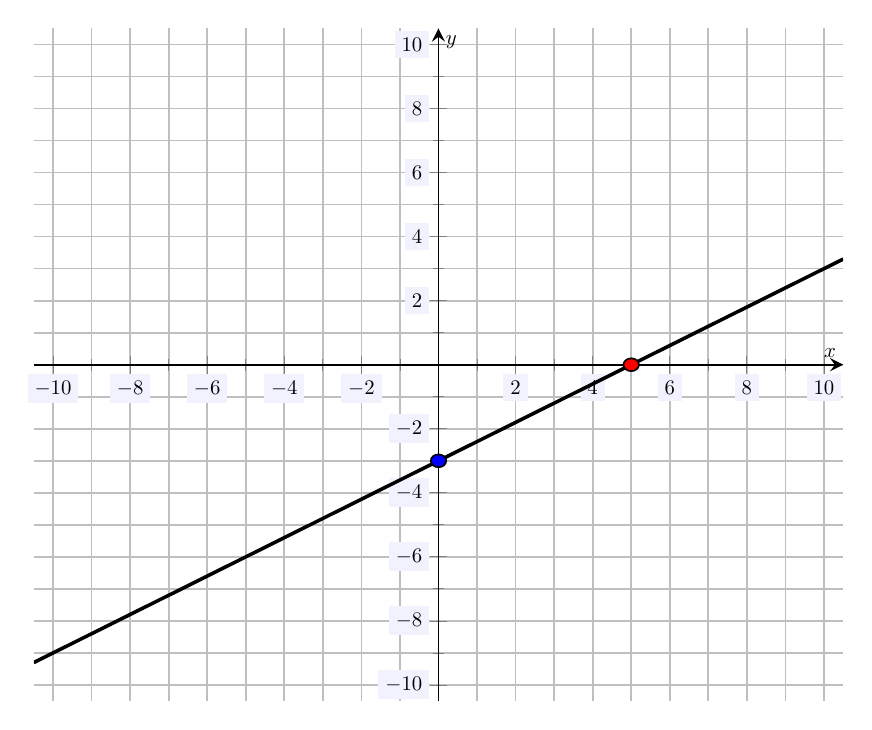
\begin{tikzpicture}[scale=1.5,every node/.style={scale=0.5}]
	\begin{axis}[
	grid=both,
	axis lines=middle,
	ticklabel style={fill=blue!5!white},
	xmin= -10.5, xmax=10.5,
	ymin= -10.5, ymax=10.5,
	xtick={-10,-8,-6,-4,-2,0,2,4,6,8,10},
	ytick={-10,-8,-6,-4,-2,0,2,4,6,8,10},
	minor tick = {-10,-9,...,10},
	xlabel=\(x\),ylabel=\(y\),
	]
	\addplot[domain=-10.5:10.5,samples=2,line width=0.03cm] (x, 3/5*x - 3);
	\draw[fill=blue] (0,-3) circle (0.2);
	\draw[fill=red] (5,0) circle (0.2);
	\end{axis}
	\end{tikzpicture}
	}
	\] \pspace

\sol We know that the line has the form $y= mx + b$. Observe that we have the point $(0, -3)$ on the line. For each increase of 5 in $x$, there is a corresponding 3 increase in $y$. Therefore, we have $m= \frac{\Delta y}{\Delta x}= \frac{3}{5}$. But then we know that $y= \frac{3}{5}\,x + b$. Using the fact that $(0, -3)$ is on the line, we have $-3= \frac{3}{5} \cdot 0 + b$ so that $b= -3$. Therefore, the line is $y= \frac{3}{5}\,x - 3$. But then $f(x)= \frac{3}{5}\,x - 3$. 

\begin{enumerate}[(a)]
\item  Because $f(x)= \frac{3}{5}\,x - 3$ has the form $y= mx + b$ with $m= \frac{3}{5}$ and $b= -3$, we know that the slope of $f(x)$ is $\frac{3}{5}$. \pspace

\item  Because $f(x)= \frac{3}{5}\,x - 3$ has the form $y= mx + b$ with $m= \frac{3}{5}$ and $b= -3$, we know that the $y$-intercept of $f(x)$ is $-3$, i.e. $(0, -3)$. Note we can also see the $y$-intercept as the marked blue point, $(0, -3)$, on the graph. \pspace

\item From the work above, we know that $f(x)= \frac{3}{5}\,x - 3$. \pspace

\item The $x$-intercept occurs when $y= 0$. But then we have\dots
	\[
	\begin{aligned}
	f(x)&= \dfrac{3}{5}\,x - 3 \\[0.3cm]
	0&= \dfrac{3}{5}\,x - 3 \\[0.3cm]
	\dfrac{3}{5}\,x&= 3 \\[0.3cm]
	\dfrac{5}{3} \cdot \dfrac{3}{5}\, x&= 3 \cdot \dfrac{5}{3} \\[0.3cm]
	x&= 5 
	\end{aligned}
	\]
Therefore, the $x$-intercept is $x= 5$, i.e. $(5, 0)$. We can also see the $x$-intercept as the red point, $(5, 0)$, marked on the graph. 
\end{enumerate}


\end{document}